\documentclass{beamer}
\usepackage{hyperref}
\usepackage{listings}
\usepackage{graphicx}
\usepackage{upquote}
\usepackage{textcomp}

\usepackage[T1]{fontenc}
\usepackage[utf8]{inputenc}

\usepackage{DejaVuSansMono}

\lstset{basicstyle=\fontfamily{dejavu}\footnotesize\ttfamily,breaklines=true}
\lstset{frame=bottomline}
\lstset{upquote=true}

\hypersetup{
  colorlinks   = true,
  linkcolor    = blue,
  citecolor    = gray
}

\usetheme{Rochester}
\title{I need a Hero(ku)} 
\subtitle{ Writing microservice daemons... in the cloud!}
\author{Andrew Ballinger}
\begin{document}

\frame{\titlepage}

\begin{frame}[fragile]
  \frametitle{Overview}

  \begin{itemize}
  \item{Microservices}
  \item{Some ideas}
  \item{Macro-micro-service providers}
  \item{To be an enemy of the state}
  \item{Live coding}
  \end{itemize}

\end{frame}

\begin{frame}[fragile]
  
  \frametitle{Microservices}
  
  Micro is small. \\ Services are things that other software uses to do stuff.

  \begin{itemize}
  \item{Less then a day}
  \item{Hosted separately}
  \item{Fire and forget}
  \end{itemize}

\end{frame}

\begin{frame}[fragile]
  
  \frametitle{Ideas}

  \begin{itemize}
  \item{Massage emails}
  \item{Send text messages}
  \item{API glue}
  \item{One-off scripts} 
  \item{Simple static website} 
  \end{itemize}

\end{frame}

\begin{frame}[fragile]
  
  \frametitle{Macro-micro-service providers}

  \begin{itemize}
  \item{Heroku}
  \item{Google App Engine}
  \item{Amazon <Blank>}
  \item{Digital Ocean} 
  \item{Vultr} 
  \item{Linode (even)} 
  \end{itemize}

\end{frame}

\begin{frame}[fragile]
  
  \frametitle{Macro-micro-service providers}

  \begin{itemize}
  \item{Heroku}
  \item{Google App Engine}
  \item{Amazon <Blank>}
  \item{Digital Ocean} 
  \item{Vultr} 
  \item{Linode (even)} 
  \end{itemize}

\end{frame}

\begin{frame}[fragile]
  \frametitle{To be an enemy of the state}

  State makes micro-services a lot harder to implement and maintain.
  
  \begin{itemize}
  \item{Persistence}
  \item{Logging}
  \item{Schema}
  \end{itemize}
  
\end{frame}

\begin{frame}[fragile]
  \frametitle{Some Relevant Comics}

   \begin{figure}[p]
    \centering
    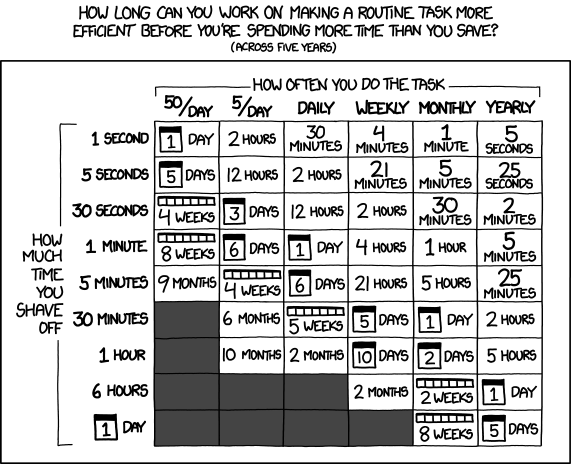
\includegraphics[height=10em]{is_it_worth_the_time.png}
    
\includegraphics[height=10em]{automation.png}
    \caption{\url{www.xkcd.com}}
  \end{figure}

\end{frame}

\begin{frame}[fragile]
  \frametitle{Let's do this}

   \begin{figure}[p]
    \centering
    
\includegraphics[width=15em]{well-do-it-live.jpg}
    \caption{Obligatory meme that dates the talk (or me)}
  \end{figure}

  \centering\href{https://devcenter.heroku.com/articles/getting-started-with-ruby#introduction}{Getting Started with Ruby on Heroku}
  
\end{frame}

\end{document}
